\newcommand{\obsvec}{y}
\newcommand{\obsymat}{H}
\newcommand{\obsx}{x}
\newcommand{\obsxmat}{A}
\newcommand{\obsdist}{w}
\newcommand{\obsvar}{R}

\newcommand{\statevec}{\alpha}
\newcommand{\statecvar}{P}
\newcommand{\statemat}{F}
\newcommand{\strdist}{v}
\newcommand{\statevar}{Q}
\newcommand{\gain}{K}
\newcommand{\statemu}{\mu}

\newcommand{\altstatevar}{B}
\newcommand{\altobsvar}{C}
\newcommand{\alldist}{\varepsilon}

\newcommand{\prederr}{e}
\newcommand{\predvar}{\Sigma}

\newcommand{\myvec}{\mbox{vec}}
\newcommand{\myvech}{\mbox{vech}}

\chapter{State Space Modeling}
\label{chap:kalman}

\section{Introduction}
\label{sec:amble}

The original interface to the treatment of linear state space models
in gretl (which has now been retired) predated the development of
gretl's ``bundle'' type.\footnote{If anyone needs documentation for
  the original interface, available in gretl 2016d and earlier
  versions, it can be found at
  \url{http://gretl.sourceforge.net/papers/kalman_old.pdf}.}  In 2016
it struck the gretl authors that the bundle type could be used to
advantage in reformulating the user interface; we suspect people will
find the new interface substantially easier to use. The new interface
makes it more practical to split long portions of code into smaller,
dedicated functions, which are arguably easier to debug and maintain;
hopefully this may lead to more function packages using gretl's native
state space facilities. Moreover, the new design is such that certain
operations that would have required a good deal of low-level coding
under the old regime are now simple, fast and natural---for example,
``disturbance smoothing'' (see section \ref{sec:kdsmooth}) or setting
up time-varying system matrices (see section \ref{sec:tvarying}).

Technically, a gretl bundle is an associative array; that is, an
all-purpose container into which you can put matrices, scalars,
strings and so on, identified by keys. A Kalman bundle is a somewhat
regimented version of the same. There are two sets of ``reserved''
keys, one set pertaining to input matrices and the other to results
generated by the Kalman functions.  Beyond that, however, you are free
to add to the bundle whatever extra elements you think may be useful.

Here are the main features of the new interface ``at a glance'':
%
\begin{itemize}
\item The Kalman structure, which used to be entirely \textit{sui
    generis}, is implemented as a bundle.
\item You can therefore have as many named models as you like in
  existence at one time, and you can pass them as arguments to
  functions.
\item The ``block'' syntax for defining a filter is replaced by the
  function \cmd{ksetup}.
\item The signatures of the functions \cmd{kfilter} and \cmd{ksmooth}
  are much simplified. For the most part you retrieve results by
  reading bundle members instead of poking in matrix-pointer
  arguments.
\item A new function, \cmd{kdsmooth}, implements Koopman's
  ``disturbance smoother.''
\item The \cmd{ksimul} function has been revamped and improved.
\item The mechanism for handling time-varying system matrices has been
  simplified and generalized.
\end{itemize}

\section{Notation}

In this document our basic representation of a state-space model is
given by the following pair of equations:
%
\begin{align}
  \label{eq:state}
  \statevec_{t+1} &= \statemat_t \statevec_t + \strdist_t \\
  \label{eq:obs}
  \obsvec_t &= \obsxmat_t'\obsx_t + \obsymat_t' \statevec_t +
  \obsdist_t 
\end{align}
%
where (\ref{eq:state}) is the state transition equation and
(\ref{eq:obs}) is the observation or measurement equation.  The state
vector, $\statevec_{t}$, is ($r \times 1$) and the vector of
observables, $\obsvec_t$, is ($n \times 1$); $\obsx_t$ is a ($k
\times 1$) vector of exogenous variables.  The ($r \times 1$) vector
$\strdist_t$ and the ($n \times 1$) vector $\obsdist_t$ are assumed to
be vector white noise:
%
\begin{align*}
E(\strdist_t \strdist_s') &= \statevar_t \mbox{ for } t = s, 
    \mbox{ otherwise } \mathbf{0} \\
E(\obsdist_t \obsdist_s') &= \obsvar_t \mbox{ for } t = s, 
    \mbox{ otherwise } \mathbf{0}
\end{align*}

The number of time-series observations is denoted by $T$.  In the case
when $\statemat_t = \statemat$, $\obsymat_t = \obsymat$,
$\obsxmat_t = \obsxmat$, $\statevar_t = \statevar$ and
$\obsvar_t = \obsvar$ for all $t$, the model is said to be
\emph{time-invariant}. We assume time-invariance in most of what
follows, but discuss the time-varying case in
section~\ref{sec:tvarying}.

\section{Defining the model as a bundle}
\label{sec:setup}

The \cmd{ksetup} function is used to initialize a state space model,
by specifying only its indispensable elements: the observables and
their link to the unobserved state vector, plus the law of motion for
the latter and the covariance matrix of its innovations. Therefore,
the function takes a minimum of four arguments.\footnote{An optional,
  fifth argument is used for initializing a state space model in which
  there is some non-zero correlation between the disturbances
  $\strdist_t$ and $\obsdist_t$. See section \ref{sec:crossd}.} The
corresponding bundle keys are as follows:

\begin{center}
\begin{tabular}{ccl}
Symbol & Dimensions & Reserved key \\[6pt]
$\obsvec$      & $T \times n$ & \texttt{obsy}\\
$\obsymat$      & $r \times n$ & \texttt{obsymat}\\
$\statemat$    & $r \times r$ & \texttt{statemat}\\
$\statevar$      & $r \times r$ & \texttt{statevar}\\
\end{tabular}
\end{center}

For example,
\begin{code}
bundle SSmod = ksetup(y, H, F, Q)
\end{code} 

The names of these input matrices don't matter; in fact they may be
anonymous matrices constructed on the fly. But if and when you wish to
copy them out of the bundle, you must use the specified keys:
\begin{code}
matrix H = SSmod.obsymat
\end{code}

Although all the arguments are in concept matrices, as a convenience
you may give \texttt{obsy} as a series or list of series, and the
other arguments can be given as scalars if in context they are
$1 \times 1$.

If applicable you may specify any of the following optional input
matrices:\footnote{An additional optional matrix is described in
section~\ref{sec:stconst} below.}

\begin{center}
\begin{tabular}{ccll}
Symbol & Dimensions & Key & If omitted\dots \\[6pt]
$\obsx$ & $T \times k$ & \texttt{obsx} &
 no exogenous terms in observation equation\\
$\obsxmat$ & $k \times n$ & \texttt{obsxmat} &
 no exogenous terms in observation equation\\ 
$\obsvar$ & $n \times n$ & \texttt{obsvar} & 
 no disturbance term in observation equation \\
$\hat{\statevec}_{1|0}$ & $r \times 1$ & \texttt{inistate} &
 $\hat{\statevec}_{1|0}$ is a zero vector\\
$\statecvar_{1|0}$ & $r \times r$ & \texttt{inivar} &
 $\statecvar_{1|0}$ is set automatically
\end{tabular}
\end{center}

However, these optional matrices are not passed to \cmd{ksetup},
rather you add them to the bundle returned by \cmd{ksetup} (under
their reserved keys) as you usually add elements to a bundle:
\begin{code}
SSmod.obsxmat = A
\end{code}

Once setup is complete the dimensions of the model, $r$, $n$, $k$ and
$T$, become available as scalar members of the bundle (under their own
names).

It might appear that the \texttt{obsx} ($\obsx$) and \texttt{obsxmat}
($\obsxmat$) matrices must go together---either both are given or
neither is given.  But an exception is granted for convenience.  If
the observation equation includes a constant but no additional
exogenous variables, you can give a ($1 \times n$) value for
$\obsxmat$ without having to specify \texttt{obsx}.  More generally,
if the row dimension of $\obsxmat$ is 1 greater than the column
dimension of $\obsx$, it is assumed that the first element of
$\obsxmat$ is associated with an implicit column of ones.

The automatic initialization of $\statecvar_{1|0}$ (in case
\texttt{inivar} is not specified) is applicable only if all the
eigenvalues of $\statemat$ lie inside the unit circle. In this case,
the variance for the marginal distribution of $\statevec_t$ is well
defined and equals
\[
\myvec(\statecvar_{1|0}) = \left[ I - \statemat \otimes \statemat
\right]^{-1} \myvec(\statevar) ,
\]
which is the formula used internally. Otherwise, we apply a diffuse
prior, setting $\statecvar_{1|0} = \kappa I_r$ with $\kappa = 10^7$.
You can impose this diffuse prior from the outset by setting a
non-zero scalar value on the bundle under the (reserved) key
\texttt{diffuse}:
%
\begin{code}
SSmod.diffuse = 1
\end{code}

\section{Special features of state-space bundles}
\label{sec:ss-special}

A bundle created by \cmd{ksetup} works in most ways like any other
gretl bundle; however, some differences should be kept in mind.  With
an ordinary bundle you can replace or delete members at will; with a
state-space bundle there are certain constraints.

\begin{itemize}
\item You can replace the coefficient matrices \texttt{obsymat},
  \texttt{statemat}, \texttt{statevar} and (if applicable)
  \texttt{obsvar} and/or \texttt{obsxmat} in a given bundle if you
  wish---but only on condition that the replacement matrix has the
  same dimensions as the original. Or in other words, the dimensions
  $r$, $n$ and $k$ are set once and for all by the initialization
  (section~\ref{sec:setup}).
\item You can replace the data matrices \texttt{obsy} and (if
  applicable) \texttt{obsx} subject to the condition that the number
  of columns is unchanged ($n$ and $k$ respectively): the time-series
  length, $T$, is mutable. But note that if \texttt{obsx} is present
  it must have at least as many rows as \texttt{obsy} (which defines
  $T$ for the bundle).
\item None of the input matrices just mentioned can be deleted from
  the bundle.
\item Output matrices that are automatically added to the bundle by
  the functions described in the following sections \textit{can} be
  deleted (if you don't need them and want to save on storage). But
  they cannot be replaced by arbitrary user content.
\item The only other ``special'' member that can be deleted is the
  function call (string) that is discussed in
  section~\ref{sec:tvarying}.
\end{itemize}

Nonetheless, in the ``user area'' of the bundle (that is, under keys
other than the reserved ones noted in this chapter), the usual rules
apply.

For all the ``\cmd{k}'' functions described below the first argument
(in most cases the only argument) must be a pointer to a bundle
obtained via \cmd{ksetup}. Any old bundle will not do. A ``pointer to
bundle'' is specified by prefixing the name of the bundle with an
ampersand, as in ``\verb|&SSmod|''. Passing the argument in pointer
form allows these functions to modify the content of the bundle.

\section{The \cmd{kfilter} function}
\label{sec:kfilter}

Once a model is established, as described in the previous section,
\cmd{kfilter} can be used to run a forward, forecasting pass.  This
function takes a single argument, namely a bundle-pointer, and it
returns a scalar code: 0 for successful completion, or non-zero if
numerical problems were encountered.

On successful completion, several elements are added to the input
bundle (or updated if they're already present).  A scalar under the
key \texttt{lnl} gives the overall log-likelihood under the joint
normality assumption,
%
\[
  \ell = -\frac{1}{2} \left[nT \log(2 \pi) + \sum_{t=1}^T\log \left|\predvar_t\right| + 
    \sum_{t=1}^T\prederr_t'\predvar_t^{-1} \prederr_t
  \right]
\]
%
and the scalar \texttt{s2} holds the estimated variance,
%
\[
\hat{\sigma}^2 = \frac{1}{nT} 
   \sum_{t=1}^T\prederr_t'\predvar_t^{-1} \prederr_t
\]
(but see section~\ref{sec:lldiffuse} below for modifications to these
formulae for the case of a diffuse prior).  The key \texttt{llt} gives
access to a $T$-vector, element $t$ of which is
%
\[
  \ell_t = -\frac{1}{2} \left[n \log(2 \pi) + \log \left|\predvar_t\right| + 
    \prederr_t'\predvar_t^{-1} \prederr_t
  \right]
\]
%

Five additional matrices also become available.  Each of these has $T$
rows, one for each time-step; the contents of the rows are shown in
the following listing.
%
\begin{enumerate}
\item Forecast errors for the observable variables, $\prederr_t'$, $n$
  columns: key \texttt{prederr}.
\item Variance matrix for the forecast errors, $\myvech(\predvar_t)'$,
  $n(n+1)/2$ columns: key \texttt{pevar}.
\item Estimate of the state vector, $\hat{\statevec}_{t|t-1}'$, $r$
  columns: key \texttt{state}.
\item MSE of estimate of the state vector,
  $\myvech(\statecvar_{t|t-1})'$, $r(r+1)/2$ columns: key \texttt{stvar}.
\item Kalman gain, $\myvec(\gain_t)'$, $rn$ columns: key
  \texttt{gain}.
\end{enumerate}

The Kalman gain is defined as 
\[
\gain_t = \statemat_t \statecvar_{t|t-1} \obsymat_t 
\left[\obsymat_t' \statecvar_{t|t-1} \obsymat_t + \obsvar_t\right]^{-1}
\]
This matrix is rarely required by the user. However, it is the key
quantity in the filtering algorithm, so we make it available under a
dedicated key for diagnostic purposes in case numerical problems
should arise. For example, the following retrieves the gain after a
filtering operation:
%
\begin{code}
kfilter(&SSmod)
matrix G = SSmod.gain
\end{code}

Then, for example, if you want to retrieve the matrix $\gain$ at time
10, you need to reshape the tenth row of the matrix \texttt{G} into
the appropriate dimensions:
\begin{code}
matrix K10 = mshape(G[10,], SSmod.r, SSmod.n)  
\end{code}

\section{The \cmd{ksmooth} function}
\label{sec:ksmooth}

Like \cmd{kfilter}, this function takes a single bundle-pointer
argument and returns an integer error code (0 indicating success).  It
runs a forward, filtering pass followed by a backward pass which
computes a smoothed estimate of the state and its MSE using the method
of Anderson and Moore.

Note that since \cmd{ksmooth} starts with a forward pass, it can be
run without a prior call to \cmd{kfilter}. This may appear to be
useless duplication, but in fact it enables an efficient scripting
option.  The main utility of the forward pass lies in the calculation
of the log-likelihood in the context of estimation; however, if a
state space model contains no parameters that have to be estimated,
the model setup can be followed directly by a call to
\cmd{ksmooth}. (And the same goes for \cmd{kdsmooth} below.)

The backward-pass algorithm is as follows: for $t=T,\dots,1$
%
\begin{align*}
L_t &= \statemat_t - \gain_t \obsymat_t' \\
u_{t-1} &= \obsymat_t \predvar_t^{-1} \prederr_t 
 + L_t' u_t \\
U_{t-1} &= \obsymat_t \predvar_t^{-1} \obsymat_t' + 
  L_t' U_t L_t \\
\hat{\statevec}_{t|T} &= \hat{\statevec}_{t|t-1} + 
  \statecvar_{t|t-1} u_{t-1} \\
\statecvar_{t|T} &= \statecvar_{t|t-1} - 
  \statecvar_{t|t-1} U_{t-1} \statecvar_{t|t-1}
\end{align*}
%
with initial values $u_T = 0$ and $U_T =
0$.\footnote{See I. Karibzhanov's clear exposition at
\url{http://karibzhanov.com/help/kalcvs.htm}.}

On successful completion, all the quantities computed by
\cmd{kfilter} are available as bundle members (see
section~\ref{sec:kfilter}), but the keys \texttt{state} and
\texttt{stvar} now give the smoothed estimates.  That is, row $t$ of
the \texttt{state} matrix holds $\hat{\statevec}_{t|T}'$ and row $t$
of \texttt{stvar} holds $\statecvar_{t|T}$, in transposed vech form
($r(r+1)/2$ elements).

\section{The \cmd{kdsmooth} function}
\label{sec:kdsmooth}

This function requires a bundle-pointer argument and returns an
integer error code (0 indicating success).  It runs a forward,
filtering pass followed by a backward pass which computes a smoothed
estimate of the disturbances along with a dispersion measure, using
the methods described in \cite{koopman93} and \cite{koopman-etal99}.

Upon successful execution of the function, the bundle will contain
under the key \texttt{smdist} a $T \times (r+n)$ matrix holding
smoothed estimates of $\strdist_t$ and $\obsdist_t$. That is, a matrix
whose $t$-th row contains
\[
(\hat{\strdist}_t' , \hat{\obsdist}_t')
 = E\left[ (\strdist_t' , \obsdist_t') \,| \,
   \obsvec_1, \ldots, \obsvec_T \right]
\]
(This assumes the observation equation has a stochastic component; if
it does not, then \texttt{smdist} is just $T \times r$.)

An associated dispersion measure is provided under the key
\texttt{smdisterr}. The precise definition of this matrix depends on a
second, optional Boolean parameter. Before describing the action of
this parameter we need to give a brief account of the two variance
measures that are found in the literature on disturbance
smoothing. Our account runs in terms of the state disturbance,
$\strdist_t$, but it applies equally to the observation disturbance,
$\obsdist_t$, if present.

One measure of variance is the mean square distance of the inferred
disturbances from zero (that is, from their unconditional
expectation). Let us call this $V^{(1)}_t$:
\[
V^{(1)}_t = E\left(\hat{\strdist}_t\hat{\strdist}_t'\right)
\]
This measure is used in computing the so-called \emph{auxiliary
  residuals}, which are advocated in \cite{durbin-koopman12} as useful
diagnostic tools. Auxiliary residuals for the state equation are
obtained by dividing $\hat{\strdist}_t$ by the square roots of the
associated diagonal elements of $V^{(1)}_t$. In computing this matrix
we use the formulae given in \citet[section 4.4]{koopman-etal99}.

A second measure of variance is the mean squared distance of the
inferred disturbances around their true values, or in other words the
mean squared error, which we'll write as $V^{(2)}_t$.
\[
V^{(2)}_t = E\left[\left(\hat{\strdist}_t - \strdist_t\right)
  \left(\hat{\strdist}_t - \strdist_t\right)'
  | \,\obsvec_1, \ldots, \obsvec_T \right]
\] 
We calculate this matrix using the formulae given in \citet[section
4.5.2]{durbin-koopman12}. Its diagonal elements can be used to form
confidence intervals for the true disturbances.

We are now ready to state what gretl provides under the key
\texttt{smdisterr}. If the optional second argument is present and
non-zero the results are based on $V^{(2)}_t$, otherwise (that is, by
default) they are based on $V^{(1)}_t$. In either case row $t$ of
\texttt{smdisterr} contains the square roots of the diagonal elements
of the matrix in question: the first $r$ elements pertain to the state
disturbances and the following $n$ elements to the observation
equation (if applicable). Like \texttt{smdist}, \texttt{smdisterr} has
$T$ rows and either $r+n$ or $r$ columns depending on whether or not
there's a disturbance term in the observation equation. We return
standard deviations rather than variances since most of the time
it's the former that users will actually want.

Section~\ref{sec:example_dsmooth} presents a script which exercises
the disturbance smoother and illustrates the difference between
$V^{(1)}_t$ and $V^{(2)}_t$.


\section{The \cmd{ksimul} function}
\label{sec:ksimul}

This simulation function has as its required arguments a pointer to a
Kalman bundle and a matrix containing artificial disturbances, and it
returns a matrix of simulation results. An optional trailing Boolean
argument is supported, the purpose of which is explained below.

If the disturbances are not cross-correlated, the matrix argument must
be either $T \times r$, if there is no disturbance in the observation
equation, or $T \times (r+n)$ if the $\obsvar$ (\texttt{obsvar})
matrix is specified. Row $t$ holds either $\strdist_t'$ or
$(\strdist_t', \obsdist_t')$. Note that if $\statevar$
(\texttt{statevar}) is not simply an identity matrix you will have to
scale the artificial state disturbances appropriately; the same goes
for $\obsvar$ and the observation disturbances, if present. Given a
matrix $U$ containing standard normal variates, in the general case
this requires finding a matrix $Z$ such that
\[
ZZ' = \Omega \equiv \left(
\begin{array}{ll}
Q & 0_{r \times n} \\
0_{n\times r} & R
\end{array}
\right)
\]
and post-multiplying $U$ by $Z'$ (although it's not necessary to form
$Z$ explicitly if the disturbance variance matrices are
diagonal). This is not particularly onerous if $\Omega$ is
time-invariant; gretl's \cmd{psdroot} function can be used to form $Z$
if it's needed. If $Q$ and/or $R$ are time-varying, however, this
scaling can become quite burdensome. As a convenience, the ancillary
function \cmd{ksimdata} can be used to pre-process the $U$ matrix
automatically. Here's an example (we assume that a bundle named
\texttt{B} has been obtained via \cmd{ksetup}):
%
\begin{code}
matrix N = mnormal(500, B.r + B.n)
matrix E = ksimdata(&B, N)
matrix sim = ksimul(&B, E)
\end{code}
%
or if you have no need to store the disturbances:
%
\begin{code}
matrix sim = ksimul(&B, ksimdata(&B, mnormal(500, B.r + B.n)))
\end{code}
%
Time-variation or no, \cmd{ksimdata} should ensure that the
disturbances are scaled to the variances specified by $Q_t$ and $R_t$.

If the disturbances are cross-correlated (see
section~\ref{sec:crossd}) then the matrix argument to \cmd{ksimul}
should be $T \times p$, each row holding $\alldist_t'$. In this case
no prior scaling is required since it is assumed that
$\alldist_t \sim N(0, I)$ and the disturbances for the respective
equations, $\altstatevar_t \alldist_t$ and $\altobsvar_t \alldist_t$,
are computed internally, with regard to time-variation if applicable.

For the purposes of \texttt{ksimul} the time-series length, $T$, is
defined by the number of rows of the supplied disturbance matrix. This
need not equal the original $T$ value (set from \texttt{obsy} in the
initial call to \cmd{ksetup}), since \texttt{obsy} is ignored under
simulation. However, if the model includes exogenous variables in the
observation equation (\texttt{obsx}) and the simulation length is
greater than the original $T$, the simulation will run out of data and
fail unless you supply a larger $x$ matrix.  This can be done in
either of two ways. You can add a suitably sized matrix to the Kalman
bundle under the key \texttt{simx}; if present, this will be used in
preference to \texttt{obsx} for simulation. Or if you don't mind
over-writing the original \texttt{obsx} you can substitute another
matrix with the required number of rows under that key.

By default, the value returned by \cmd{ksimul} is a ($T \times n$)
matrix holding simulated values for the vector of observables at each
time step; that is, row $t$ holds $\tilde{\obsvec}_t'$, where the tilde
indicates a simulated quantity.  To obtain a record of the simulated
state, supply a non-zero value for the final, optional argument. In
that case the returned matrix is $T \times (r+n)$ and contains both
the simulated state and the simulated observable; row $t$ holds
$(\tilde{\statevec}_t', \tilde{\obsvec}_t')$.

Note that the original \texttt{obsy} member of the bundle is not
overwritten by \texttt{ksimul}, nor is \texttt{state} or any other
user-accessible output matrix. On exit from \texttt{ksimul} the prior
$T$ value is restored.

The recursion that yields $\tilde{\obsvec}$ and $\tilde{\statevec}$
is as follows: for $t=1,\dots,T$
%
\begin{align*}
  \tilde{\obsvec}_t &= \obsxmat_t'\obsx_t + 
   \obsymat_t' \tilde{\statevec}_t + \obsdist_t  \\ 
  \tilde{\statevec}_{t+1} &= \statemat_t \tilde{\statevec}_t + \strdist_t
\end{align*}
%
This implies that a value for $\tilde{\statevec}_1$ is required to get
things started. You can add such a value to a Kalman bundle under the
reserved key \texttt{simstart}. If this member is not present in the
bundle, $\tilde{\statevec}_1$ defaults to the value given under the
key \texttt{inistate}, or if that in turn is not present, to a zero
vector. A further note on initializing the state can be found in
section~\ref{sec:simstart}.

% \textbf{IDEA}: it would be very nice to find a simple case to
% exemplify this in a bootstrap context, along the lines of 
% \cite{stoffer-wall91}.

\section{Some finer points}
\label{sec:finer}

\subsection{Cross-correlated disturbances}
\label{sec:crossd}

The formulation given in equations (\ref{eq:state}) and (\ref{eq:obs})
assumes mutual independence of the disturbances in the state and
observation equations, $\strdist_t$ and $\obsdist_t$.  This assumption
holds good in many practical applications, but a more general
formulation allows for cross-correlation.  In place of
(\ref{eq:state})--(\ref{eq:obs}) we may write
%
\begin{align*}
  \statevec_{t+1} &= \statemat_t \statevec_t + 
     \altstatevar_t \alldist_t \\
  \obsvec_t &= \obsxmat_t'\obsx_t + \obsymat_t' \statevec_t + 
     \altobsvar_t \alldist_t 
\end{align*}
%
where $\alldist_t$ is a ($p \times 1$) disturbance vector which is
assumed to satisfy $\alldist_t \sim N(0, I_p)$, $\altstatevar_t$ is
($r \times p$) and $\altobsvar_t$ is ($n \times p$).

For example, the special case where $\altobsvar = I$ is referred to as
``innovations representation'' in \cite{hansen-sargent2013} and is a
cornerstone of a sizeable strand of literature in contemporary
macroeconomics.

In terms of input syntax, if the state and observation disturbances
are cross-correlated five arguments should be given to the
\cmd{ksetup} function (see section~\ref{sec:setup}): in place of
giving $\statevar$ you should give the two matrices identified above as
$\altstatevar$ and $\altobsvar$, as in
\begin{code}
bundle SSxmod = ksetup(y, H, F, B, C)
\end{code}

In case you wish to retrieve or update information on the variance of
the disturbances, note that in the cross-correlated case the bundle
keys \texttt{statevar} and \texttt{obsvar} are taken to designate the
factors $\altstatevar$ and $\altobsvar$ respectively.

\subsection{Intercept in the state equation}
\label{sec:stconst}

In some applications it is useful to be able to have an ``intercept''
in the state transition equation, thus generalizing equation
\eqref{eq:state} to
\[
  \statevec_{t+1} = \statemu_t + \statemat_t \statevec_t + \strdist_t \\
\]
The term $\statemu$ is never strictly necessary: the system
(\ref{eq:state}) and (\ref{eq:obs}) without $\statemu$ is general
enough to accommodate such a term, by absorbing it as an extra (non
time-varying) element in the state vector.  However, this comes at the
cost of expanding all the matrices that touch the state ($\statevec$,
$\statemat$, $\strdist$, $\statevar$, $\obsymat$), making the model
relatively awkward to formulate and forecasts more expensive to
compute. Therefore, we adopt the convention above on practical
grounds.

The ($r \times 1$) vector $\statemu$ can be specified as a bundle
member by the name \texttt{stconst}. Despite its name, this matrix can
be stipulated as time varying, as explained in the next section.

\subsection{Time-varying matrices}
\label{sec:tvarying}

Any or all of the matrices \texttt{obsymat}, \texttt{obsxmat},
\texttt{obsvar}, \texttt{statemat}, \texttt{statevar} and
\texttt{stconst} may be time-varying.  In that case you must supply
the name of a function to be called to update the matrix or matrices
in question: you add this to the bundle as a string, under the key
\texttt{timevar\_call}.\footnote{The choice of the name for the
  function itself is of course totally up to the user.} For example,
if just \texttt{obsymat} ($\obsymat_t$) should be updated, by a
function named \texttt{TV\_H}, you would write
%
\begin{code}
SSmod.timevar_call = "TV_H"
\end{code}
%
The function that plays this role will be called at each time-step of
the filtering or simulation operation, prior to performing any
calculations. It should have a single bundle-pointer parameter, by
means of which it will be passed a pointer to the Kalman bundle to
which the call is attached.  Its return value, if any, will not be
used, so generally it returns nothing (is of type \cmd{void}).
However, you can use gretl's \texttt{funcerr} keyword to raise an
error if things seem to be going wrong; see
chapter~\ref{chap:functions} for details.

Besides the bundle members noted above, a time variation function has
access to the current (1-based) time step, under the reserved key
\texttt{t}, and the $n$-vector containing the forecast error from the
previous time step, $\prederr_{t-1}$, under the key \texttt{uhat};
when $t=1$ the latter will be a zero vector.

If any additional information is needed for performing the update it
can be placed in the bundle under a user-specified key.  So, for
example, a simple updater for a ($1 \times 1$) $\obsymat$ matrix might
look like this:
%
\begin{code}
function void TV_H (bundle *b)
    b.obsymat = b.Hvals[b.t]
end function
\end{code}
%
where \texttt{b.Hvals} is a bundled $T$-vector. An updater that
operates on both $\obsymat$ ($r \times n$) and $\statemat$ ($r \times
r$) might be
%
\begin{code}
function void update_2 (bundle *b)
    b.obsymat = mshape(b.Hvals[b.t,], b.r, b.n)
    b.statemat = unvech(b.Fvals[b.t,])
end function
\end{code}
%
where in this case we assume that \texttt{b.Hvals} is $T \times rn$,
with row $t$ holding the (transposed) vec of $\obsymat_t$, and
\texttt{b.Fvals} is $T \times r(r+1)/2$, with row $t$ holding the vech
of $\statemat_t$. Simpler variants (e.g.\ just one element of a
relevant matrix in question is changed) and more complex
variants---say, involving some sort of conditionality---are also
possible in this framework.

It is worth noting that this setup lends itself to a much wider scope
than time-varying system matrices. In fact, this syntax allows for the
possibility of executing user-defined operations at each step. The
function that goes under \texttt{timevar\_call} can read all the
elements of the model bundle and can modify several of them: the
system matrices (which can therefore be made time-varying) as well as
the user-defined elements.

An extended example of use of the time-variation facility is presented
in section~\ref{sec:ss-examples}.

\subsection{Likelihood under the diffuse prior}
\label{sec:lldiffuse}

This note pertains to the \cmd{kfilter} function (see
section~\ref{sec:kfilter}). 

There seems to be general agreement in the literature that the
log-likelihood calculation should be modified in the case of a diffuse
prior for $\statecvar_{1|0}$.  However, it is not clear to us that
there is a well-defined ``correct'' method for this.  At present we
emulate \textsf{SsfPack}.  In case
$\statecvar_{1|0} = \kappa I_r$, we set $d = r$ and calculate
%
\[
  \ell = -\frac{1}{2} \left[(nT-d) \log(2 \pi) + 
    \sum_{t=1}^T\log \left|\predvar_t\right| + 
    \sum_{t=1}^T\prederr_t'\predvar_t^{-1} \prederr_t
    - d \log(\kappa)
  \right]
\]
%
and
%
\[
\hat{\sigma}^2 = \frac{1}{nT-d} 
   \sum_{t=1}^T\prederr_t'\predvar_t^{-1} \prederr_t
\]

\subsection{The initial state under simulation}
\label{sec:simstart}

We pointed out in section~\ref{sec:ksimul} above that you can specify
the initial state, $\statevec_1$, from which recursion starts under
simulation via the bundle key \texttt{simstart}. If you wish to make
this starting point stochastic, you can emulate the procedure followed
by \textsf{SsfPack}, namely setting
\[
\alpha_1 = a + Z v_0
\]
where $a$ is a non-stochastic $r$-vector, $v_0$ is an $r$-vector
of standard normal random numbers, and $Z$ is a matrix such
that $ZZ' = \statecvar_{1|0}$.

Let's say we have a state-space bundle \texttt{B}, on which we have
already set suitable values of \texttt{inistate} (corresponding to $a$
above) and \texttt{inivar} ($\statecvar_{1|0}$).  Now we want to
perform a simulation with a stochastic starting point. In hansl we
could set $\alpha_1$ thus:
%
\begin{code}
matrix Z = psdroot(B.inivar)
B.simstart = B.inistate + Z * mnormal(B.r, 1)
\end{code}

\section{Example scripts}
\label{sec:ss-examples}

This section presents a selection of short sample scripts to
illustrate the most important points covered in this chapter.

\subsection{ARMA estimation}
\label{sec:example_arma}

Functions illustrated in this example: \cmd{ksetup}, \cmd{kfilter}.

As is well known, the Kalman filter provides a very efficient way to
compute the likelihood of ARMA models; as an example, take an
ARMA(1,1) model
\[
  y_t = \phi y_{t-1} + \varepsilon_t + \theta \varepsilon_{t-1}
\]
One of the ways the above equation can be cast in state-space form is
by defining a latent process $\xi_t = (1 - \phi L)^{-1}
\varepsilon_t$.   The observation equation corresponding to (\ref{eq:obs})
is then
%
\begin{equation}
y_t = \xi_t + \theta \xi_{t-1} \label{eq:arma-meas}
\end{equation}
%
and the state transition equation corresponding to (\ref{eq:state}) is
%
\[
  \left[ \begin{array}{c} \xi_t \\ \xi_{t-1} \end{array} \right] =
  \left[ \begin{array}{cc} \phi & 0 \\ 1 & 0 \end{array} \right]
  \left[ \begin{array}{c} \xi_{t-1} \\ \xi_{t-2} \end{array} \right] +
  \left[ \begin{array}{c} \varepsilon_t \\ 0 \end{array} \right] 
\]

The \textsf{hansl} syntax for a corresponding filter would be
\begin{code}
matrix H = {1; theta}
matrix F = {phi, 0; 1, 0}
matrix Q = {s^2, 0; 0, 0}
bundle kb = ksetup(y, H, F, Q)
\end{code}
%
or, if you prefer, just a one-liner:
\begin{code}
bundle kb = ksetup(y, {1; theta}, {phi, 0; 1, 0}, {s^2, 0; 0, 0})
\end{code}

Note that the observation equation (\ref{eq:arma-meas}) does not
include an ``error term''; this is equivalent to saying that
$\mbox{var}(\obsdist_t) = 0$ and there is therefore no need to add
an \texttt{obsvar} element to the bundle.

Once the filter is set up, all it takes to compute the log-likelihood
for given values of $\phi$, $\theta$ and $\sigma^2_{\varepsilon}$ is
to execute the \cmd{kfilter} function and read the Kalman
bundle's \texttt{lnl} member (which holds the total log-likelihood)
or, more appropriately if the likelihood has to be maximized through
\cmd{mle}, \texttt{llt}, which gives the series of individual
contribution to the log-likelihood for each observation. An example is
shown in script~\ref{script:armaest}.

\begin{script}[htbp]
  \caption{ARMA estimation}
  \label{script:armaest}
\begin{scode}
function void arma11_via_kalman (series y)
    /* parameter initialization */
    scalar phi = 0
    scalar theta = 0
    scalar sigma = 1
    
    /* state-space model setup */
    matrix H = {1; theta}
    matrix F = {phi, 0; 1, 0}
    matrix Q = {sigma^2, 0; 0, 0}
    bundle kb = ksetup(y, H, F, Q)
    
    /* maximum likelihood estimation */
    mle logl = ERR ? NA : kb.llt
        kb.obsymat[2] = theta
        kb.statemat[1,1] = phi
        kb.statevar[1,1] = sigma^2
        ERR = kfilter(&kb)
        params phi theta sigma
    end mle --hessian
end function

# ------------------------ main ---------------------------

open arma.gdt        # open the "arma" example dataset
arma11_via_kalman(y) # estimate an arma(1,1) model
arma 1 1 ; y --nc    # check via native command
\end{scode}
\end{script}

\subsection{Local level model}
\label{sec:example_loclev}

Functions illustrated in this example: \cmd{ksetup}, \cmd{kfilter},
\cmd{ksmooth}.

Suppose we have a series $y_t = \mu_t + \varepsilon_t$, where $\mu_t$
is a random walk with normal increments of variance $\sigma^2_1$ and
$\varepsilon_t$ is normal white noise with variance $\sigma^2_2$,
independent of $\mu_t$. This is known as the ``local level'' model,
and it can be cast in state-space form as equations
(\ref{eq:state})-(\ref{eq:obs}) with $\statemat = 1$,
$\strdist_t \sim N(0,\, \sigma^2_1)$, $\obsymat = 1$ and
$\obsdist_t \sim N(0,\, \sigma^2_2)$.  The translation to
\textsf{hansl} is
\begin{code}
bundle llmod = ksetup(y, 1, 1, s1)
llmod.obsvar = s2
llmod.diffuse = 1
\end{code}

The two unknown parameters $\sigma^2_1$ and $\sigma^2_2$ can be
estimated via maximum likelihood.  Script~\ref{script:loclev} provides
an example of simulation and estimation of such a model. Since
simulating the local level model is trivial using ordinary gretl
commands, we don't use \cmd{ksimul} in this context.\footnote{Warning:
  the way the script is, there is an ``off-by-one'' misalignment
  between the state vector and the observable series. For convenience,
  the script is written as if equation \eqref{eq:state} was modified
  into the equivalent formulation
  \[
  \statevec_{t} = \statemat \statevec_{t-1} + \strdist_t ;
  \]
  we tried to keep the script as simple as possible, so that the
  reader is free to focus on the interesting aspects. }

\begin{script}[htbp]
  \caption{Local level model}
  \label{script:loclev}
\begin{scode}
nulldata 200
set seed 101010
setobs 1 1 --special-time-series

/* set the true variance parameters */
true_s1 = 0.5
true_s2 = 0.25

/* and simulate some data */
v = normal() * sqrt(true_s1)
w = normal() * sqrt(true_s2)
mu = 2 + cum(v)
y = mu + w

/* starting values for variance estimates */
s1 = 1
s2 = 1

/* state-space model set-up */
bundle kb = ksetup(y, 1, 1, s1)
kb.obsvar = s2
kb.diffuse = 1

/* ML estimation of variances */
mle ll = ERR ? NA : kb.llt
    ERR = kfilter(&kb)
    params kb.statevar kb.obsvar
end mle

/* compute the smoothed state */
ksmooth(&kb)
series muhat = kb.state
\end{scode}
\end{script}

\subsection{Time-varying models}
\label{sec:example_PhCurve}

In order to illustrate state space models with time-varying system
matrices, we will use time-varying OLS. Suppose the DGP for an
observable time series $y_t$ is given by
\begin{equation}
  \label{eq:tvarols-1}
    y_t = \beta_0 + \beta_{1,t} x_t + \varepsilon_t
\end{equation}
where the slope coefficient $\beta_1$ evolves through time according to
\begin{equation}
  \label{eq:tvarols-2}
    \beta_{1,t+1} = \beta_{1,t} + \eta_t
\end{equation}

It is easy to see that the pair of equations above define a state
space model, with equation \eqref{eq:tvarols-1} as the measurement
equation and \eqref{eq:tvarols-2} as the state transition equation. In
other terms, $\beta_{1,t}$ is the unobservable state, $\statemat = 1$
and $\statevar = V(\eta_t) = \sigma^2_{\eta}$; as for the measurement
equation, $\obsvar = V(\varepsilon_t) = \sigma^2_{\varepsilon}$, but
the matrix multiplying $\beta_{1,t}$, and hence $\obsymat$, is $x_t$,
which is clearly time-varying.

\begin{figure}[htbp]
  \centering
    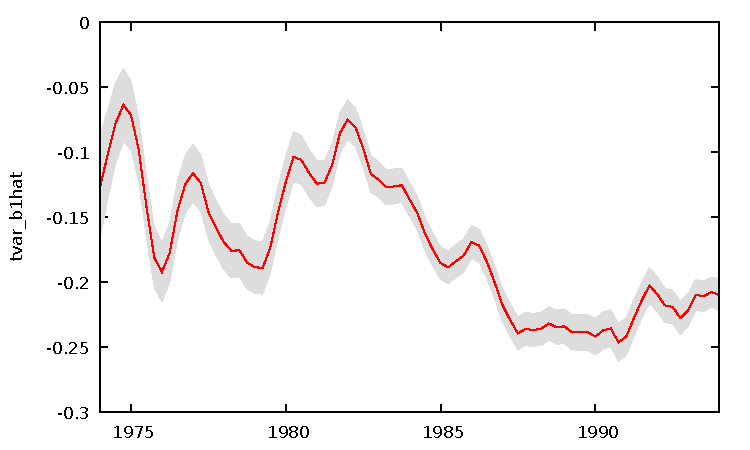
\includegraphics{figures/timevar_PhCurve} \\[10pt]
  \caption{Phillips Curve on Euro data: time-varying slope and
    95\% confidence interval}
  \label{fig:tvar}
\end{figure}

Once the system is framed as a state-space model, estimation of the
three unknown parameters $\beta_0$, $\sigma^2_{\varepsilon}$ and
$\sigma^2_{\eta}$ may proceed by maximum likelihood in a manner
similar to example \ref{script:armaest} and \ref{script:loclev}. The
sequence of slope coefficients $\beta_{1,t}$ is, instead, estimated by
running the smoother, which also yields a consistent estimate of the
dispersion of the estimated state

Script \ref{script:PhCurve} presents an example of the above, in which
data from the AWM database are used to estimate a Phillips Curve
with time-varying slope:
\[
\mbox{INFQ}_t = \beta_0 + \beta_{1,t} \mbox{URX}_t + \varepsilon_t
\]
where INFQ is a measure of quarterly inflation and URX a measure of
unemployment.  At the end of the script, the evolution through time of
the slope coefficient is plotted together with a 95\% confidence
band---see Figure~\ref{fig:tvar}.

\begin{script}[htbp]
  \caption{Phillips curve on Euro data with time-varying slope}
  \label{script:PhCurve}
\begin{scode}
function void at_each_step(bundle *b)
    b.obsymat = transp(b.mX[b.t,])
end function

open AWM.gdt --quiet
smpl 1974:1 1994:1

/* parameter initialization */
scalar b0 = mean(INFQ)
scalar s_obs = 0.1
scalar s_state = 0.1

/* bundle setup */
bundle B = ksetup(INFQ, 1, 1, 1)
matrix B.mX = {URX}
matrix B.depvar = {INFQ}
B.timevar_call = "at_each_step"
B.diffuse = 1

/* ML estimation of intercept and the two variances */
mle LL = err ? NA : B.llt
    B.obsy = B.depvar - b0
    B.obsvar = s_obs^2
    B.statevar = s_state^2
    err = kfilter(&B)
    params b0 s_obs s_state
end mle

/* display the smoothed time-varying slope */
ksmooth(&B)
series tvar_b1hat = B.state[,1]
series tvar_b1se = sqrt(B.stvar[,1])
gnuplot tvar_b1hat --time-series --with-lines --output=display \
    --band=tvar_b1hat,tvar_b1se,1.96 --band-style=fill
\end{scode}
\end{script}

\subsection{Disturbance smoothing}
\label{sec:example_dsmooth}

Functions illustrated in this example: \cmd{ksetup}, \cmd{kdsmooth}.

In section~\ref{sec:kdsmooth} we noted that the \cmd{kdsmooth}
function can produce two different measures of the dispersion of the
smoothed disturbances, depending on the the value of the (optional)
trailing Boolean parameter. Here we show what these two measures are
good for, using the famous Nile flow data that have been much analysed
in the state-space modeling literature. We focus on the state
equation; that is, the random-walk component of the observed series.
For consistency with the literature let us call the $t$-dated
disturbance to the state $\eta_t$.

In the first call to \cmd{kdsmooth} we omit the optional switch and
therefore compute $E(\hat{\eta}_t\hat{\eta}_t')$ for each $t$. This
quantity is suitable for constructing the auxiliary residuals shown in
the top panel of Figure~\ref{fig:nile} (for similar plots see
\cite{koopman-etal99}, \cite{pelagatti11}).  This plot suggests the
presence of a structural break shortly prior to 1900, as various
authors have observed.

In the second \cmd{kdsmooth} call we ask gretl to compute instead
$E[(\hat{\eta}_t-\eta_t)(\hat{\eta}_t-\eta_t)' | y_1,\ldots,y_T]$, the
MSE of $\hat{\eta}_t$ considered as an estimator of $\eta_t$. And in
the lower panel of the Figure we plot $\hat{\eta}_t$ along with a 90\%
confidence band (roughly, $\pm 1.64$ times the RMSE). This reveals
that, given the sampling variance of $\hat{\eta}_t$, we're not really
sure that any of the $\eta_t$ values were truly different from
zero. The resolution of the seeming conflict here is commonly reckoned
to be that there was in fact a change in mean around 1900, but besides
that event there's little evidence for a non-zero
$\sigma^2_{\eta}$. Or in other words the standard local level model is
not really applicable to the data.


\begin{script}[htbp]
  \caption{Working with smoothed disturbances -- Nile data}
  \label{script:auxres}
\begin{scode}
open nile.gdt

# ML variance estimates
scalar s2_eta = 1468.49
scalar s2_eps = 15099.7

bundle LLM = ksetup(nile, 1, 1, s2_eta)
LLM.obsvar = s2_eps
LLM.diffuse = 1

kdsmooth(&LLM)
series eta_aux = LLM.smdist[,1] ./ LLM.smdisterr[,1]
series zero = 0
plot eta_aux
    options time-series with-lines band=zero,const,2
    option band-style=dash
    literal set ylabel ''
    literal set title 'Auxiliary residual, state equation'
end plot --output=display

kdsmooth(&LLM, 1)
series etahat = LLM.smdist[,1]
series sdeta = LLM.smdisterr[,1]

plot etahat
    options time-series with-lines band=etahat,sdeta,1.64485
    option band-style=dash
    literal set ylabel ''
    literal set title 'State disturbance with 90% confidence band'
end plot --output=display
\end{scode}
\end{script}

\begin{figure}[htbp]
  \centering
  \begin{tabular}{cc}
  \small
  (a) Auxiliary (standardized) residuals, state equation \\
    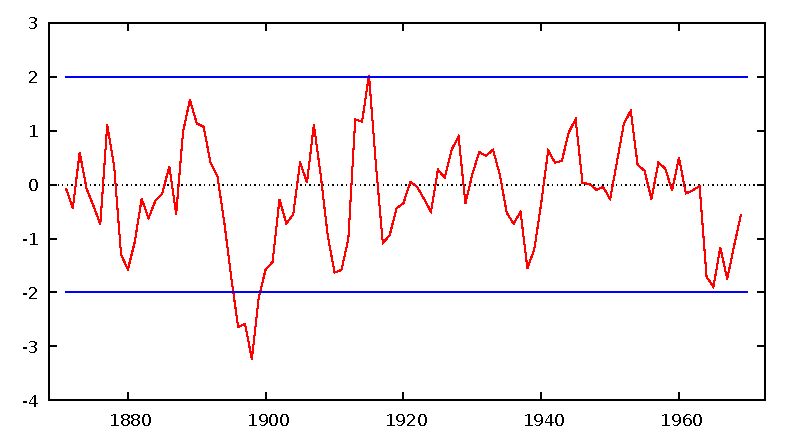
\includegraphics{figures/nile_eta_ksd} \\[14pt]
  \small (b) Estimated state disturbance with 90\% confidence band \\
  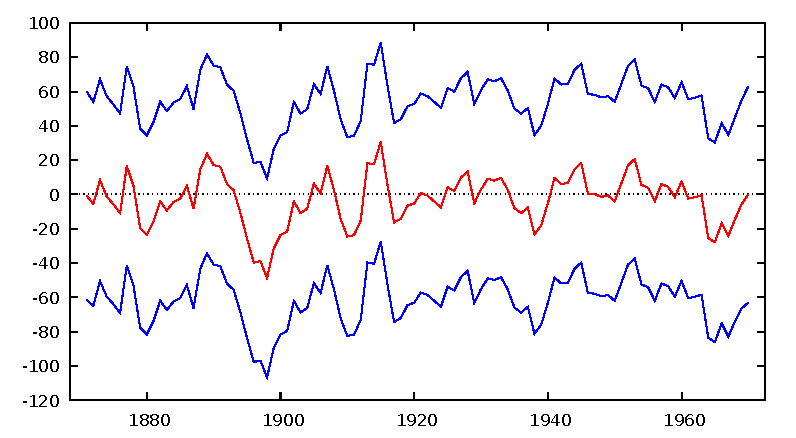
\includegraphics{figures/nile_eta_dk}
  \end{tabular}
  \caption{Nile data: auxiliary residuals and $\hat{\eta}_t$
    from disturbance smoother}
  \label{fig:nile}
\end{figure}
